\section{Case Studies}
\label{sec:case-studies}

%------------------------------------------------

In the sequel, three case studies are described in depth to exemplify the main features of the tool.
First, \sref{sec:eval-prerequisites} discusses the prerequisite analysis features of the tool, and presents a summary of statistics about the universities included in this study.
Second, \sref{sec:eval-topics} closely considers two areas within Computer Science and discusses the inferred topics for courses within those areas.
Finally, \sref{sec:eval-comparison} details the similarities and differences between pairs of university departments and also presents a summary of comparisons between all the universities in this study.

%------------------------------------------------

%\begin{table}[ht]
%\centering
%\begin{tabular}{lll}
%\toprule
%& Jaccard & Percent \\
%\midrule
%mean   & 0.145 & 0.229 \\
%median & 0.156 & 0.217 \\
%\midrule
%max    & 0.007 & 0.007 \\
%min    & 0.311 & 0.709 \\
%\bottomrule
%\end{tabular}
%\caption{Evaluation of all result sets\label{tbl:evaluation-before}}
%\end{table}

%------------------------------------------------

%\begin{table}[ht]
%\centering
%\begin{tabular}{lll}
%\toprule
%& Jaccard & Percent \\
%\midrule
%mean   & 0.203 & 0.377\\
%median & 0.206 & 0.351\\
%\midrule
%max    & 0.058 & 0.082\\
%min    & 0.311 & 0.709\\
%\bottomrule
%\end{tabular}
%\caption{Evaluation of result sets with more than one predicted knowledge area on average per course\label{tbl:evaluation-after}}
%\end{table}

%------------------------------------------------

\subsection{Case Study: Prerequisite Analysis}
\label{sec:eval-prerequisites}

%------------------------------------------------

To understand how a course fits into a department, its position in the prerequisite chain must be analyzed.
Take, for example, a course in mobile application development.
We predict that any course of this nature will most likely be an upper level elective with a moderate number of prerequisite courses.
Indeed, we see this is the case with George Mason's CS 477, Portland State's CS 410, and Stanford's 231M.
However, many of the topics covered in a mobile development course are niche topics, and specific to that field.
Therefore, it might not be the case that any particular lower level courses will cover specific, overlapping topics.

%------------------------------------------------

Let us consider George Mason University's CS 477 ``Mobile Application Development''.
The course description discusses mobile platforms and the various software design issues specific to mobile platforms.
There are two inferred topics for this course.
The first topic, with 32\% proportion, includes the terms ``develop'', ``platform'', and ``mobile'' at high frequency.
The second topic, with only 15\% proportion, is more generic and includes terms like ``system'', ``computer'', and ``topic''.
The course also has two registered prerequisites: CS 310 ``Data Structures'' and CS 367 ``Computer Systems and Programming''.
Within the context of the department, these two courses are major prerequisites for any upper level course.
As expected, neither of the two prerequisite courses share the mobile-specific topic inferred for CS 477.
CS 310, however, does overlap with the generic computer systems topic.
We therefore conclude that the CS 477 course registers its prerequisites primarily to ensure a baseline level of maturity and skill among its students, rather than because some necessary concepts are introduced at a lower level and expanded upon at the higher level.

%------------------------------------------------

To quantify the typical level of conceptual overlap between prerequisites within a department, we introduce a vector representation of a course, the ``weighted topic-vector''.
Like the unweighted topic-vector representation of a department, the weighted topic-vector is a vector of uniform length corresponding to the total number of inferred topics among all known courses.
However, the features of a weighted topic-vector represent the proportion with which the particular topic is represented in the course's description.
In this way, the weighted topic-vector takes into account the importance of a topic to a course, rather than simply binary topic membership as in the unweighted topic-vector.
By computing the average distance between the weighted topic-vectors of a course and its prerequisites, the level of conceptual overlap for that course can be quantified.
Averaging these distance measures over every course in the department that has registered prerequisites results in a measure of average prerequisite conceptual overlap within the department.
\tref{tbl:prereq-topic-overlap} summarizes the levels of conceptual overlap for the five universities in the dataset with registered prerequisite trees, where a higher average value of conceptual overlap indicates a closer relationship between courses and their prerequisites.
The five universities not included did not have prerequisite relationships in their collected data, and thus this analysis could not be performed.

%------------------------------------------------

\begin{table}
  \centering
  \begin{tabular}{rcc}
    \toprule
     & Prereq$_\mu$ & Prereq$_\sigma$ \\
    \midrule
    GMU  & 0.324 & 0.211 \\
    AU   & 0.278 & 0.134 \\
    KSU  & 0.273 & 0.213 \\
    Utah & 0.257 & 0.249 \\
    UTK  & 0.201 & 0.256 \\
    \bottomrule
  \end{tabular}
  \caption{Level of conceptual overlap between courses and their prerequisites in five universities. Prereq$_\mu$ is the average level of conceptual overlap between prerequisites, Prereq$_\sigma$ is the standard deviation.\label{tbl:prereq-topic-overlap}}
\end{table}

%------------------------------------------------

\subsection{Case Study: Topics In Computer Science}
\label{sec:eval-topics}

%------------------------------------------------

\subsubsection{Ethics In Computer Science}
\label{sec:eval-topics-ethics}

%------------------------------------------------

Computer Science is a wide ranging field, with a number of disparate subfields --- according to the \ac{acm}, there are 18 distinct Knowledge Areas~\cite{CS2013}.
At any given university, the Computer Science department will, ideally, cover all or most of these areas.
One particular area covered by most universities in this study is ``Social Issues and Professional Practice''.
A clear example of a course within this Knowledge Area is any course in computing and ethics.
Take, for example, Kansas State's CIS 415 ``Ethics and Computing Technology.''
The description is brief and to the point, focusing on computing ethics within a professional context.
The only topic inferred for this course, at 64\% proportion, includes the terms ``ethics'', ``computer'', ``profession'', ``issue'', and ``social'' at high frequency.
Searching for other courses that teach to the same topic yields 30 courses across nine universities (every university in the study except for Rensselaer Polytechnic).
These courses have titles like ``Computer Ethics and Society'' (GMU CS 105) and ``Ethics in Computing'' (LSU CSC 1200).
This demonstrates the ability of our tool to not only automatically infer relevant concepts from a course description, but to match related courses across universities.

%------------------------------------------------

\subsubsection{Artificial Intelligence}
\label{sec:eval-topics-ai}

%------------------------------------------------

Another major topic within computer science is the study of \ac{ai}.
\ac{ai} itself contains a great number of subfields and areas of specialization, but it is defined in \ac{acm} Knowledge Area ``Intelligent Systems'' as ``the study of solutions for problems that are difficult or impractical to solve with traditional methods''~\cite{CS2013}.
Consider Portland State's CS 441 ``Artificial Intelligence.''
Its course description is highly typical of \ac{ai} courses included in this study: brief and to the point, it lists a number of subfields within \ac{ai} that will be touched upon in the course.
The only topic inferred for this course, at 86\% proportion, includes the terms ``intelligence'', ``knowledge'', ``artificial'', and ``agent'' at high frequencies.
Every other university in this study also contains at least one course which teaches to this topic in some proportion.
George Mason's CS 480 ``Introduction to Artificial Intelligence'', Louisiana State's CSC 4444 ``Artificial Intelligence'' and University of Utah's CS 6380 ``Multi-Agent Systems'' to name a few.
Indeed, many of these courses share very similar descriptions.

%------------------------------------------------

However, one of the most unique examples of a course with this topic is the University of Tennessee's COSC 420 ``Biologically-Inspired Computation.''
The title alone might not suggest that this is an \ac{ai} based class, and indeed it is not entirely \ac{ai}.
The course description talks about swarm intelligences, multi-agent systems, and other biomimetic computational systems.
While the common \ac{ai} topic discussed prior is inferred at 42\%, two other topics, one with terms from biology and one with terms from neural networks, a subfield of \ac{ai}, appear at proportions 24\% and 17\% respectively.
UTK's COSC 420 is an excellent example of \ac{lda}'s ability to infer many possibly unrelated topics in a mixture within a document in order to represent the full nature of the text.

%------------------------------------------------

\subsection{Case Study: Comparing Departments}
\label{sec:eval-comparison}

%------------------------------------------------

\subsubsection{George Mason vs Stanford}
\label{sec:eval-comparison-stanford}

%------------------------------------------------

While institutions generally cover a wide range of topics, there are always certain topics that cannot be or are not taught.
Take for example George Mason University and Stanford University.
The two computer science departments share a lot in common.
Of 68 total topics covered between the two, 41 are common to both while only 14 are unique to Stanford and 13 unique to George Mason.
The shared topics contain terms that directly relate to similar courses at each school.
For example ``secure'' and ``network'' are terms in a topic taught in network security classes at both schools.
However, a topic containing ``linux'', ``unix'', ``lab'' appears unique to Stanford, covered by CS 1U ``Practical Unix'', a course that does not exist at George Mason.
Similarly, a topic containing ``parallel'' and ``algorithm'' appears unique to George Mason.
The course GMU CS 683 ``Parallel Algorithms'' teaches to this topic, with no analogous course at Stanford.

%------------------------------------------------

By analyzing the set of unique and shared topics within two departments, simple coefficients can be computed to quantify the degree of similarity.
The Jaccard coefficient is computed as the most basic representation of departmental similarity, along with Euclidean and cosine similarity metrics discussed in \sref{sec:vis-compare}.
A pairwise comparison of the universities in this study is presented in \fref{fig:heatmap}.
In this figure, darker shades of blue represent a higher degree of similarity.
Also see \tref{tbl:heatmap-key} for the specific computed similarity values.

%------------------------------------------------

\subsubsection{George Mason vs ACM EC}
\label{sec:eval-comparison-acmec}

%------------------------------------------------

The \ac{ec} provide a wide view of different courses from institutions around the world.
If we assume the \ac{ec} to compose a single, hypothetical university's CS department, we can compare existing departments against it in the same fashion as was used in \sref{sec:eval-comparison-stanford}.
Take George Mason University, for example, to compare against the \ac{ec}.
Both departments share a great deal in common, with 38 overlapping topics.
There are additionally not that many topics unique to the two departments, with 14 unique to the \ac{ec} and 18 unique to GMU.
A number of interesting artifacts appear, however, upon closer inspection.

%------------------------------------------------

Two topics unique to the \ac{ec} include the terms ``moral'' and ``religious'', one each.
Inspecting these topics reveals two members of the \ac{ec} with the titles ``Ethics \& the Information Age'' and ``Technology, Ethics, and Global Society''.
Both of these courses teach ethics in computation, but from a vastly different perspective than the ethics course at George Mason.
These two \ac{ec} ethics courses include professional ethics, but also moral, religious, and social philosophies of ethical behavior, while the George Mason ethics courses (\eg\ CS 105 ``Computer Ethics and Society'') only discuss professional ethics.
This is an important yet subtle distinction to make, which might be overlooked by simply considering course titles.

%------------------------------------------------

Another unique topic to the \ac{ec} includes the terms ``design'', ``circuit'', and ``digital''.
The courses which teach to this topic, across institutions, are primarily digital design and logic courses.
Inspecting the George Mason CS curriculum reveals that an analogous course is required within the CS degree, ECE 301 ``Digital Electronics'', but is not contained within the CS department, unlike some other universities.
This particular artifact appears because the scope of our data sets include only CS departments.
We make the assumption that necessary courses to the CS program at an institution will fall under the heading of Computer Science, which in this case is not true.

%------------------------------------------------

Note that included in \fref{fig:heatmap} are the \ac{acm} \ac{ec}.
Each course from the \ac{ec} was entered into the dataset along with every other university course, and had topics inferred by \ac{lda} in the same manner.
In this way the \ac{ec} act as control courses with a ground truth label set.
High similarity to the \ac{ec} indicates a high degree of compliance with \ac{acm} standards.

%------------------------------------------------

\begin{figure}
  \centering
  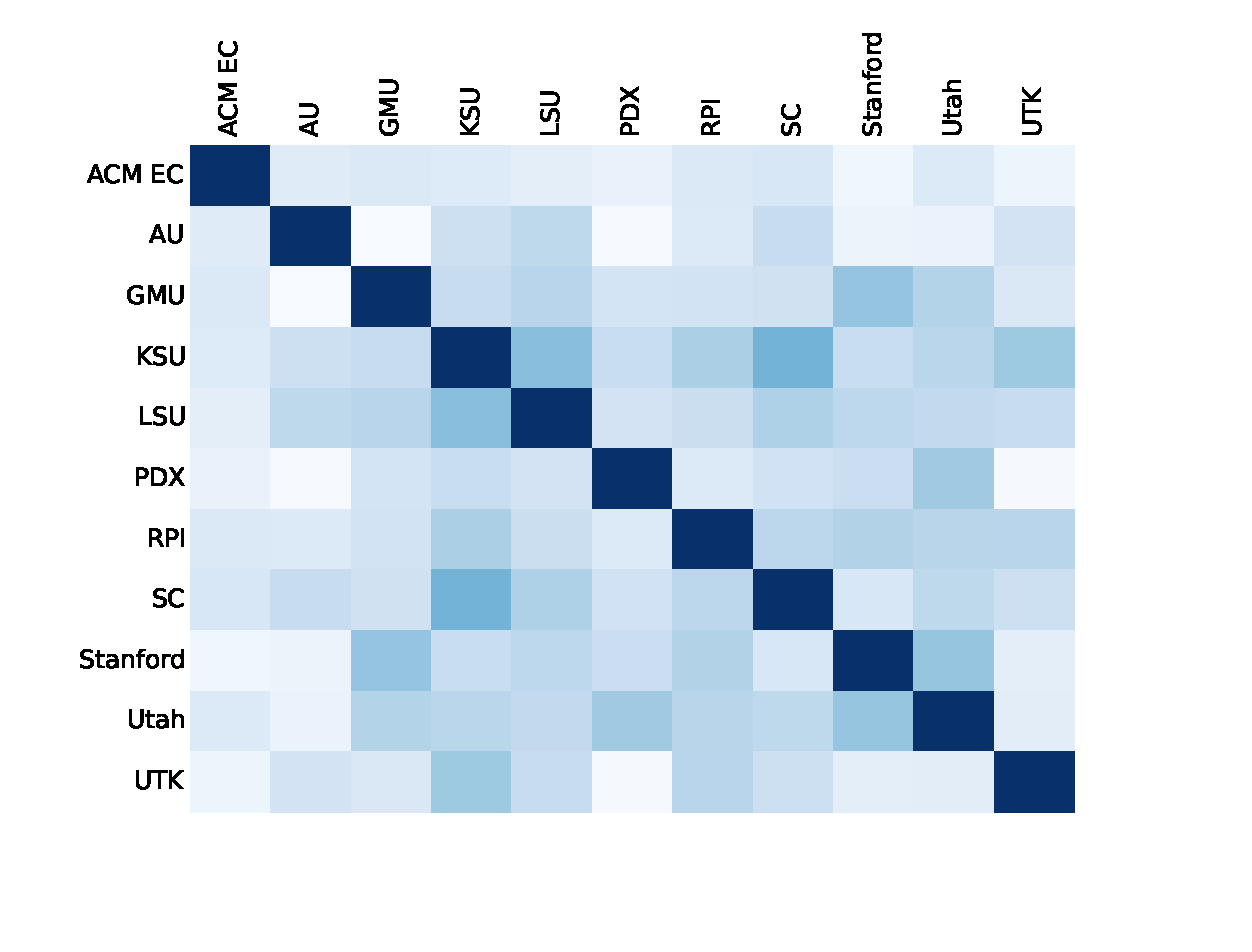
\includegraphics[width=0.5\textwidth]{figures/10by10heatmap}
  \caption{Pairwise similarity of CS departments using the Jaccard index. Darker shades indicate higher similarity. ACM EC refers to the \acf{ec}. See \tref{tbl:heatmap-key} for the specific recorded values.\label{fig:heatmap}}
\end{figure}

%------------------------------------------------

\begin{table*}
  \centering
  \begin{tabular}{lccccccccccc}
    \toprule
    & ACM EC & AU & GMU & KSU & LSU & PDX & RPI & SC & Stanford & Utah & UTK \\
    \midrule
    ACM EC & 1.000 & 0.420 & 0.433 & 0.426 & 0.407 & 0.386 & 0.433 & 0.443 & 0.366 & 0.427 & 0.373 \\
    AU & 0.420 & 1.000 & 0.339 & 0.480 & 0.522 & 0.342 & 0.431 & 0.500 & 0.377 & 0.382 & 0.462 \\
    GMU & 0.433 & 0.339 & 1.000 & 0.500 & 0.532 & 0.460 & 0.463 & 0.471 & 0.603 & 0.545 & 0.439 \\
    KSU & 0.426 & 0.480 & 0.500 & 1.000 & 0.623 & 0.494 & 0.561 & 0.655 & 0.493 & 0.528 & 0.587 \\
    LSU & 0.407 & 0.522 & 0.532 & 0.623 & 1.000 & 0.462 & 0.491 & 0.554 & 0.524 & 0.514 & 0.500 \\
    PDX & 0.386 & 0.342 & 0.460 & 0.494 & 0.462 & 1.000 & 0.427 & 0.469 & 0.488 & 0.586 & 0.347 \\
    RPI & 0.433 & 0.431 & 0.463 & 0.561 & 0.491 & 0.427 & 1.000 & 0.525 & 0.547 & 0.535 & 0.532 \\
    SC & 0.443 & 0.500 & 0.471 & 0.655 & 0.554 & 0.469 & 0.525 & 1.000 & 0.443 & 0.521 & 0.480 \\
    Stanford & 0.366 & 0.377 & 0.603 & 0.493 & 0.524 & 0.488 & 0.547 & 0.443 & 1.000 & 0.600 & 0.407 \\
    Utah & 0.427 & 0.382 & 0.545 & 0.528 & 0.514 & 0.586 & 0.535 & 0.521 & 0.600 & 1.000 & 0.409 \\
    UTK & 0.373 & 0.462 & 0.439 & 0.587 & 0.500 & 0.347 & 0.532 & 0.480 & 0.407 & 0.409 & 1.000 \\
    \bottomrule
  \end{tabular}
  \caption{Pairwise similarity of CS departments computed as Jaccard index of department topic sets.\label{tbl:heatmap-key}}
\end{table*}

%------------------------------------------------
